\documentclass[tikz, margin=3mm]{standalone}
\usepackage[colorlinks]{hyperref}

\usepackage{bbm}
\usepackage{amsmath}
\usepackage{amsfonts}
\usetikzlibrary{fit}
\usetikzlibrary{shapes.misc, positioning}
\usetikzlibrary{shapes}
\usetikzlibrary{arrows}
\usetikzlibrary{positioning}
\usetikzlibrary{calc}
\usetikzlibrary{decorations.pathreplacing}
\usetikzlibrary{decorations.pathmorphing}

\DeclareMathOperator*{\argmin}{arg\,min}
\newcommand{\Plus}{\mathord{
\begin{tikzpicture}[baseline=0ex, line width=3, scale=0.25]
\draw (1,0) -- (1,2);
\draw (0,1) -- (2,1);
\end{tikzpicture}}}

\newcommand{\PlusSmall}{\mathord{
\begin{tikzpicture}[baseline=0ex, line width=2, scale=0.10]
\draw (1,0) -- (1,2);
\draw (0,1) -- (2,1);
\end{tikzpicture}}}

\newcommand{\Minus}{\mathord{
\begin{tikzpicture}[baseline=0ex, line width=3, scale=0.25]
\draw (0,1) -- (2,1);
\end{tikzpicture}}}

\newcommand{\MinusSmall}{\mathord{\begin{tikzpicture}[baseline=0ex, line width=2, scale=0.10]
\draw (0,1) -- (2,1);
\end{tikzpicture}}}

\tikzset{weird fill/.style={append after command={
   \pgfextra
        \draw[sharp corners, fill=#1]% 
    (\tikzlastnode.west)% 
    [rounded corners=3pt] |- (\tikzlastnode.north)% 
    [rounded corners=1pt] -| (\tikzlastnode.east)% 
    [rounded corners=1pt] |- (\tikzlastnode.south)% 
    [rounded corners=3pt] -| (\tikzlastnode.west);
   \endpgfextra}}}





\begin{document}

 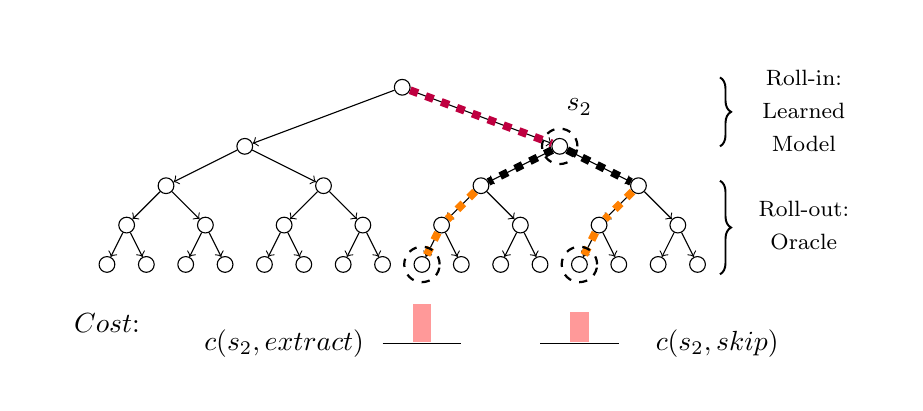
\begin{tikzpicture}
   \tikzstyle{sent}=[align=left]
   \tikzstyle{doc}=[rectangle,rounded corners,draw=black, very thick]

   \draw[white] (-1,-1.5) rectangle (10,3);

   \node at (6.,2.0) {$s_2$};
\node[draw,circle,minimum size=.20cm,inner sep=0pt] (a) at (0,0) {};
\node[draw,circle,minimum size=.20cm,inner sep=0pt] (b) at (.5,0) {};
\node[draw,circle,minimum size=.20cm,inner sep=0pt] (c) at (1,0) {};
\node[draw,circle,minimum size=.20cm,inner sep=0pt] (d) at (1.5,0) {};
\node[draw,circle,minimum size=.20cm,inner sep=0pt] (e) at (2,0) {};
\node[draw,circle,minimum size=.20cm,inner sep=0pt] (f) at (2.5,0) {};
\node[draw,circle,minimum size=.20cm,inner sep=0pt] (g) at (3,0) {};
\node[draw,circle,minimum size=.20cm,inner sep=0pt] (h) at (3.5,0) {};
\node[draw,circle,minimum size=.20cm,inner sep=0pt] (i) at (4,0) {};
\node[draw,circle,minimum size=.20cm,inner sep=0pt] (j) at (4.5,0) {};
\node[draw,circle,minimum size=.20cm,inner sep=0pt] (k) at (5,0) {};
\node[draw,circle,minimum size=.20cm,inner sep=0pt] (l) at (5.5,0) {};
\node[draw,circle,minimum size=.20cm,inner sep=0pt] (m) at (6,0) {};
\node[draw,circle,minimum size=.20cm,inner sep=0pt] (n) at (6.5,0) {};
\node[draw,circle,minimum size=.20cm,inner sep=0pt] (o) at (7,0) {};
\node[draw,circle,minimum size=.20cm,inner sep=0pt] (p) at (7.5,0) {};

\node[draw,circle,minimum size=.20cm,inner sep=0pt] (q) at (.25,.5) {};
\node[draw,circle,minimum size=.20cm,inner sep=0pt] (r) at (1.25,.5) {};
\node[draw,circle,minimum size=.20cm,inner sep=0pt] (s) at (2.25,.5) {};
\node[draw,circle,minimum size=.20cm,inner sep=0pt] (t) at (3.25,.5) {};
\node[draw,circle,minimum size=.20cm,inner sep=0pt] (u) at (4.25,.5) {};
\node[draw,circle,minimum size=.20cm,inner sep=0pt] (v) at (5.25,.5) {};
\node[draw,circle,minimum size=.20cm,inner sep=0pt] (w) at (6.25,.5) {};
\node[draw,circle,minimum size=.20cm,inner sep=0pt] (x) at (7.25,.5) {};

\node[draw,circle,minimum size=.20cm,inner sep=0pt] (y) at (.75,1) {};
\node[draw,circle,minimum size=.20cm,inner sep=0pt] (z) at (2.75,1) {};
\node[draw,circle,minimum size=.20cm,inner sep=0pt] (1) at (4.75,1) {};
\node[draw,circle,minimum size=.20cm,inner sep=0pt] (2) at (6.75,1) {};

\node[draw,circle,minimum size=.20cm,inner sep=0pt] (3) at (1.75,1.5) {};
\node[draw,circle,minimum size=.20cm,inner sep=0pt] (4) at (5.75,1.5) {};

\node[draw,circle,minimum size=.20cm,inner sep=0pt] (5) at (3.75,2.25) {};
%\node[] at ($(x) + (.75,0)$) [] {\footnotesize Sent. 4};
%\node[] at ($(x) + (.75,.5)$) [] {\footnotesize Sent. 3};
%\node[] at ($(x) + (.75,1)$) [] {\footnotesize Sent. 2};
%\node[] at ($(x) + (.75,1.75)$) [] {\footnotesize Sent. 1};

\draw[->] (5) -- (3); 
\draw[->] (5) -- (4);


\draw[->] (3) -- (y);
\draw[->] (3) -- (z);

\draw[->] (4) -- (1);
\draw[->] (4) -- (2);


\draw[->] (y) -- (q);
\draw[->] (y) -- (r);

\draw[->] (z) -- (s);
\draw[->] (z) -- (t);

\draw[->] (1) -- (u);
\draw[->] (1) -- (v);

\draw[->] (2) -- (w);
\draw[->] (2) -- (x);

\draw[->] (q) -- (a);
\draw[->] (q) -- (b);

\draw[->] (r) -- (c);
\draw[->] (r) -- (d);

\draw[->] (s) -- (e);
\draw[->] (s) -- (f);

\draw[->] (t) -- (g);
\draw[->] (t) -- (h);

\draw[->] (u) -- (i);
\draw[->] (u) -- (j);

\draw[->] (v) -- (k);
\draw[->] (v) -- (l);

\draw[->] (w) -- (m);
\draw[->] (w) -- (n);

\draw[->] (x) -- (o);
\draw[->] (x) -- (p);

\begin{pgflowlevelscope}{\pgftransformscale{0.25}}
\draw [decorate,decoration={brace,amplitude=16pt,mirror,raise=4pt,},
       line width=.1cm,yshift=0pt]
($(31,-.5)$) -- ($(31,4.25)+(0,0)$) node [black,midway,xshift=0.8cm] {};
\end{pgflowlevelscope}
\begin{pgflowlevelscope}{\pgftransformscale{0.25}}
\draw [decorate,decoration={brace,amplitude=16pt,mirror,raise=4pt,},
       line width=.1cm,yshift=0pt]
($(31,6)$) -- ($(31,9.5)+(0,0)$) node [black,midway,xshift=0.8cm] {};
\end{pgflowlevelscope}
\node[text width=1.8cm] at ($(x) + (1.6,1.45)$) [align=center] 
    {\footnotesize Roll-in: Learned Model};

\node[text width=2cm] at ($(x) + (1.6,0)$) [align=center] 
    {\footnotesize Roll-out: Oracle};


  \node[draw,circle,minimum size=.45cm,inner sep=0pt,dashed,thick] at (4) {}; 
  \draw[-,color=purple,very thick,dashed,line width=0.1cm] (5) -- (4); 
  \draw[-,color=orange,very thick,dashed,line width=0.1cm] (1) -- (u); 
  \draw[-,color=orange,very thick,dashed,line width=0.1cm] (u) -- (i); 

  \draw[-,color=black,very thick,dashed,line width=0.1cm] (4) -- (2); 
  \draw[-,color=black,very thick,dashed,line width=0.1cm] (4) -- (1); 
  \draw[-,color=orange,very thick,dashed,line width=0.1cm] (2) -- (w); 
  \draw[-,color=orange,very thick,dashed,line width=0.1cm] (w) -- (m); 

  \node at ($(a)+(0,-.75)$) [] {$Cost$:};
  \draw[-] ($(i)+(-.5,-1)$) -- ($(i)+(.5,-1)$) 
   node[midway,rectangle,text height=.25cm,fill=red!40,yshift=.26cm] (xx) {};
  \draw[-] ($(m)+(-.5,-1)$) -- ($(m)+(.5,-1)$) 
   node[midway,rectangle,text height=.15cm,fill=red!40,yshift=.21cm] (xx) {};
   \node at ($(i)+(-1.75,-1)$) [] {$c(s_2,extract)$};
   \node at ($(m)+(1.75,-1)$) [] {$c(s_2,skip)$};
  
  \node[draw,circle,minimum size=.45cm,inner sep=0pt,dashed,thick] at (i) {}; 
  \node[draw,circle,minimum size=.45cm,inner sep=0pt,dashed,thick] at (m) {}; 


\end{tikzpicture}
\end{document}
